\documentclass[onecolumn]{article}
%\usepackage{url}
%\usepackage{algorithmic}
\usepackage[a4paper]{geometry}
\usepackage{datetime}
\usepackage[margin=2em, font=small,labelfont=it]{caption}
\usepackage{graphicx}
\usepackage{mathpazo} % use palatino
\usepackage[scaled]{helvet} % helvetica
\usepackage{microtype}
\usepackage{amsmath}
\usepackage{subfigure}
% Letterspacing macros
\newcommand{\spacecaps}[1]{\textls[200]{\MakeUppercase{#1}}}
\newcommand{\spacesc}[1]{\textls[50]{\textsc{\MakeLowercase{#1}}}}

\title{\spacecaps{Assignment Report 1: Process and Thread Implementation}\\ \normalsize \spacesc{CENG2034, Operating Systems} }

\author{Zeynep Hazal Cengiz\\zeynephazalcengiz@posta.mu.edu.tr}
%\date{\today\\\currenttime}
\date{\today}

\begin{document}
\maketitle

\subsection*{Github Page}
\url{https://github.com/zeynephazal} 

\section{Introduction}

In this project, we will first create a child process with syscall. Then we will print the PIDs of it. Then we will download the files of the URL links provided with the child processes that we created

\section{Assignments}


\subsection{IMPORT}

\includegraphics[scale=0.9]{İMPORT.PNG}

\subsection*{Note} % the star suppresses numbering of sections and subsections
In this section, the necessary modules to be used in the system are imported.

\subsection{Search Dublicated Files}

\includegraphics[scale = 0.60]{DUBLİCATED.PNG}
\subsection*{Note} % the star suppresses numbering of sections and subsections
We created two hashes on behalf of photoName and photoHash. Then we drop the pictures from the links into photoHash with the help of a function.
We create a function called dltDuplicates and delete the duplicate files out of it.

\subsection{Child Processes and PID value}

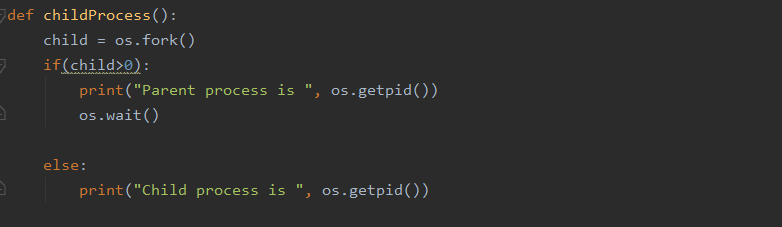
\includegraphics[scale =0.80]{child.PNG}
\subsection*{Note} % the star suppresses numbering of sections and subsections
In this section, we create a childProcess function and get the PIDs of each file.

\subsection{Dowload Files}
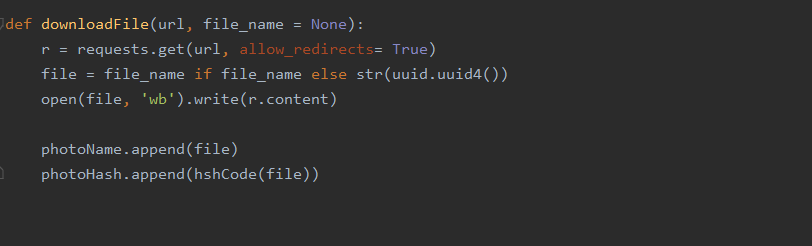
\includegraphics[scale = 0.80]{dowload.PNG}
\subsection*{Note} % the star suppresses numbering of sections and subsections
We download the url links provided with the childprocesses we created.
\subsection{Dowload Urls}
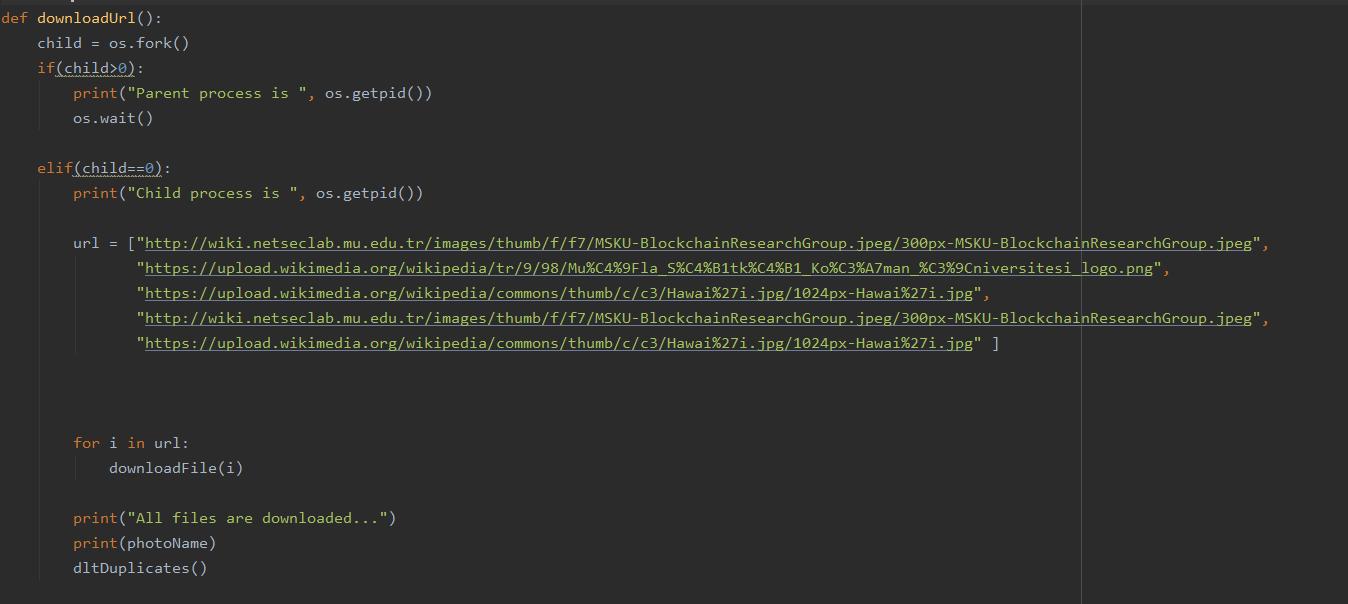
\includegraphics[scale =0.60]{last.PNG}
\subsection*{Note} % the star suppresses numbering of sections and subsections
It takes the url links given into the child process and downloads. Then we print these files.


\section{Conclusion}
We took the links of url files given in this project and put them in a childprocess. Then we downloaded these files. We delete the duplicate files from the files we downloaded. We use the "os.wait" command to get rid of the orphan process situation mentioned in question 3.


\nocite{*}
\bibliographystyle{plain}
\bibliography{references}
\end{document}